\chapter{Realization}
\minitoc
\newpage

\setcounter{secnumdepth}{0} % Set the section counter to 0 so next section is not counted in toc
% ----------------------- Introduction ----------------------- %
\section{Introduction}
A project can always look simple from the outside, however if we dive deeply into how most software is made, we can see that it's not that simple of a process.
Therefore, this chapter will list all of the technologies that we've used and also some of the major technical difficulties we've come in contact with during the realization of our project.

\setcounter{secnumdepth}{2} % Resume counting the sections for the toc with a depth of 2 (Sections and sub-sections)
% ----------------------------------- SECTIONS (v) ----------------------------------- %
% ----------------------- Technologies ----------------------- %
\section{Technologies}
This part is reserved for the presentation of all of the software used in the realization of the project and includes but is not limited to; programming languages, frameworks, technologies, etc...

\begin{itemize}
    \item \textbf{Jupyter Notebook:} \newline \cite{wikipedia} Project Jupyter is a project to develop open-source software, open standards, and services for interactive computing across multiple programming languages. \newline
          \begin{minipage}{\linewidth}
              \centering
              
\includegraphics[width=3cm]{src/assets/logos/jupyter_notebook.jpg}
              \captionof{figure}{Logo of Jupyter Notebook}
          \end{minipage}
    \item \textbf{Python Virtual Environments:} \newline A Python Virtual Environment is a self-contained environment that allows you to maintain separate package installations for different projects. \newline \newline
          \begin{minipage}{\linewidth}
              \centering
              
\includegraphics[width=6cm]{src/assets/logos/python_virtualenv.png}
              \captionof{figure}{Logo of Python Virtual Environments}
          \end{minipage}
          \newpage

    \item \textbf{Flask:} \newline Flask is a micro web framework written in Python. It is classified as a microframework because it does not require particular tools or libraries. \newline \newline
          \begin{minipage}{\linewidth}
              \centering
              
\includegraphics[width=5cm]{src/assets/logos/flask.png}
              \captionof{figure}{Logo of Flask}
          \end{minipage}
    \item \textbf{Postgres:} \newline PostgreSQL, also known as Postgres, is a free and open-source relational database management system emphasizing extensibility and SQL compliance. \newline \newline
          \begin{minipage}{\linewidth}
              \centering
              
\includegraphics[width=8cm]{src/assets/logos/postgresql.png}
              \captionof{figure}{Logo of Postgres}
          \end{minipage}
    \item \textbf{Postgres Anonymize:} \newline Postgres Anonymize is a tool for anonymizing data in a PostgreSQL database. It's useful for creating anonymized data dumps for testing and development purposes. \newline \newline
          \begin{minipage}{\linewidth}
              \centering
              
\includegraphics[width=6cm]{src/assets/logos/postgresql_anonymizer.png}
              \captionof{figure}{Logo of Postgres Anonymize}
          \end{minipage}
          \newpage

    \item \textbf{Visual Studio Code:} \newline Visual Studio Code (VSCode) is a Microsoft open-source crossplatform code editor. \newline \newline
          \begin{minipage}{\linewidth}
              \centering
              
\includegraphics[width=2.5cm]{src/assets/logos/vscode_512x512.png}
              \captionof{figure}{Logo of VSCode}
          \end{minipage}
    \item \textbf{Docker:} \newline A set of platform as a service (PaaS) products that use OS-level virtualization to deliver software in packages called containers. \newline \newline
          \begin{minipage}{\linewidth}
              \centering
              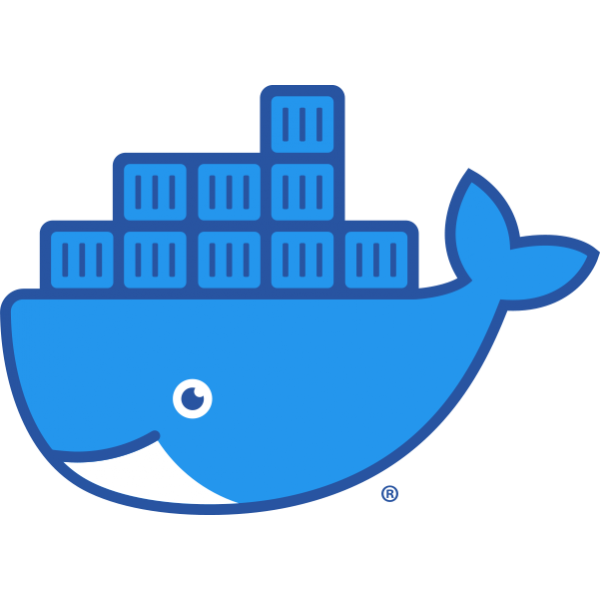
\includegraphics[width=3.5cm]{src/assets/logos/docker_512x512.png}
              \captionof{figure}{Logo of Docker}
          \end{minipage}
    \item \textbf{Docker compose:} \newline A helper tool to run applications with multiple Docker containers using a yaml format. Often used in development. \newline \newline
          \begin{minipage}{\linewidth}
              \centering
              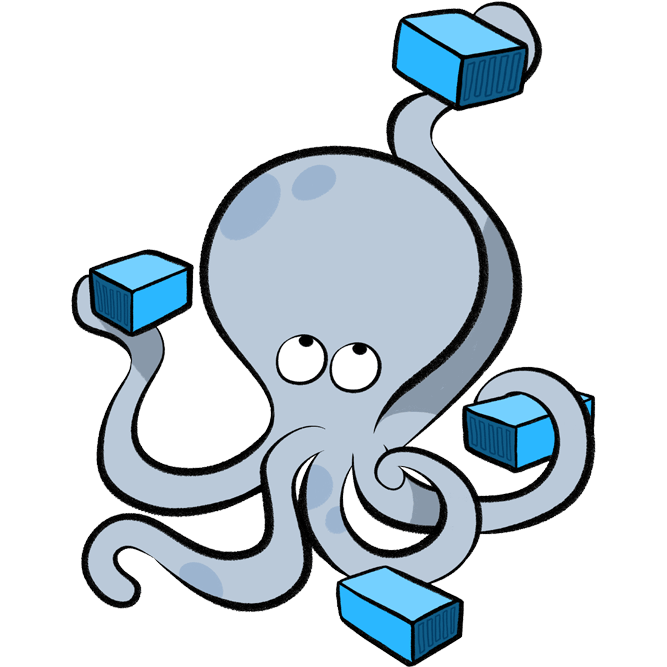
\includegraphics[width=4cm]{src/assets/logos/docker-compose_667x667.png}
              \captionof{figure}{Logo of Docker Compose}
          \end{minipage}
          \newpage

    \item \textbf{Task:} \newline A task runner / build tool that aims to be simpler and easier to use than, for example, GNU Make. \newline \newline
          \begin{minipage}{\linewidth}
              \centering
              
\includegraphics[width=3cm]{src/assets/logos/task_500x500.png}
              \captionof{figure}{Logo of Task}
          \end{minipage}
    \item \textbf{Linux:} \newline A Unix-like operating system for common daily use and more commonly for servers. \newline
          \begin{minipage}{\linewidth}
              \centering
              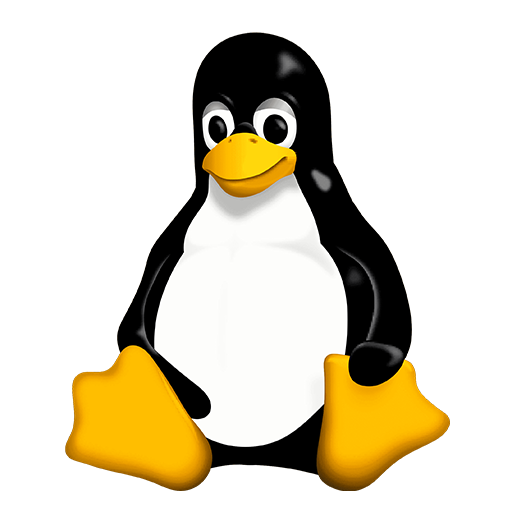
\includegraphics[width=3cm]{src/assets/logos/linux_512x512.png}
              \captionof{figure}{Logo of Linux}
          \end{minipage}
    \item \textbf{LaTeX:} \newline \cite{latex-project} A high-quality document preparation and typesetting system for technical grade documents. \newline \newline
          \begin{minipage}{\linewidth}
              \centering
              \includegraphics[width=3cm]{src/assets/logos/latex_200x200.png}
              \captionof{figure}{Logo of The LaTeX Project}
          \end{minipage}
          \newpage

\end{itemize}

% ----------------------- Deployment process ----------------------- %
\section{Deployment process}
In order to make the trained model usable by the end user, we had setup quite a few thins:

\begin{itemize}
    \item \textbf{Pickle:} Export the trained model and save it as a serializable object using the pickle library.
    \item \textbf{Flask:} Create a web server using the Flask framework to serve the model.
\end{itemize}

After that, an API endpoint that accepts the lead's id and returns the recommended messages is created.

Since this is a proof of concept, we didn't really deploy the model to a production server, but the process would be the same as deploying any other Flask app.

% ----------------------- Difficulties encountered ----------------------- %
\section{Difficulties encountered}

\subsection{Collecting the data}
The first difficulty that we've encountered was collecting the data.
The data was stored in a PostgreSQL database and we had to write a script to extract it and save it as multiple CSV files.
Not only that, but because the data contained sensitive information, we had to anonymize it before using it.

Additionally, automating the process of extracting and anonymizing the data was a challenge in itself.
In fact, at the time of writing this report, the process is still not fully automated, mostly because of the lack of time.

\setcounter{secnumdepth}{0} % Set the section counter to 0 so next section is not counted in toc
% ----------------------- Conclusion ----------------------- %
\section{Conclusion}
In this chapter, we listed all of the technology stack that we used for our app as well as some of the most weighty issues we've encountered.
We also discussed how we plan to deploy the model to a production server.
